\section{Aufbau und Durchführung}
\label{sec:Durchführung}
Im folgenden wird kurz der Aufbau des verwendeten He-Ne-Lasers erklärt und kurz die Versuchsdurchführung wiedergegeben.

\subsection{Justierung des He-Ne-Lasers}
Zu Beginn wird der Spiegel, welcher weiter von dem Justierlaser weg stehen soll (siehe Abbildung \eqref{fig:Aufbau}), auf die Schiene gesetzt und die Reflektion soll auf die Mitte des Fadenkreuzes justiert werden. Danach wird der zweite Spiegel von dem Resonator aufgestellt und erneut justiert. Als letztes wird das Laserrohr zwischen die beiden Spiegel gestellt und das Lasermedium wird durch einen Hochspannungsgenerator zu der Besetzungsinversion angeregt. Es wird solange an den Justierschrauben gedreht, bis der charakteristische rote Laser zu sehen ist. Allerdings muss der Laser noch optimiert werden, dazu wird eine Photodiode ganz ans Ende der Schiene gesetzt. Dadurch kann die Strahlintensität gemessen werden und muss durch nachjustieren der Spiegel und des Laserrohres maximiert werden.

\begin{figure}[H]
  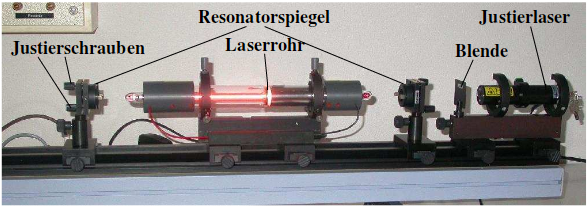
\includegraphics[width=\linewidth]{Bilder/Aufbau.png}
  \caption{Aufbau des verwendeten He-Ne-Lasers. \cite{V61}}
  \label{fig:Aufbau}
\end{figure}

\subsection{Bestimmung der Polarisation}
Um die Polarisation zu bestimmen, wird ein Polarisationsfilter zwischen die Photodiode und den Resonator gestellt. Daraufhin wird die Intensität in Abhängigkeit des Polarisationswinkels gemessen und notiert.

\subsection{Bestimmung der Wellenlänge}
Für die Bestimmung der Wellenlänge wird der Polarisationsfilter wieder entfernt und durch ein Gitter mit 100 Linien pro mm ersetzt. Dann wird die Entfernung zwischen dem Gitter und dem Schirm so groß wie möglich gewählt und notiert. Zuletzt werden die Abstände der Nebenmaxima zu dem Hauptmaximum gemessen.

\subsection{Beobachtung der TEM}
Um die TEM beobachten zu können, wird ein dünner Wolfram Draht ($0.005$mm) zwischen Resonatorspiegel und Laserrohr gestellt. Die TEM$_{00}$ (siehe Abbildung \eqref{fig:TEM00}) wird ausgemessen ohne den Draht in den Laser zu halten. Um die TEM$_{10}$ zu messen, wird der Draht in den Laser gestellt und so lange durch den Strahl bewegt, bis sich ein Bild ergibt wie in Abbildung \eqref{fig:TEM10} zu sehen ist. Bei beiden Moden soll die Intensität in Abhängigkeit zu der optischen Achse gemessen werden.

\begin{figure}
  \centering
  \begin{subfigure}[c]{0.4\textwidth}
    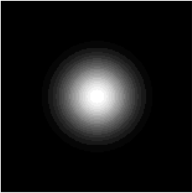
\includegraphics[width=\textwidth]{Bilder/TEM00.png}
    \caption{TEM$_{00}$-Mode}
    \label{fig:TEM00}
  \end{subfigure}
  \begin{subfigure}[c]{0.4\textwidth}
    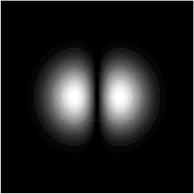
\includegraphics[width=\textwidth]{Bilder/TEM10.png}
    \caption{TEM$_{10}$-Mode}
    \label{fig:TEM10}
  \end{subfigure}
  \caption{Die ersten beiden TEM-Moden eines He-Ne-Lasers. \cite{TEM}}
\end{figure}

\subsection{Überprüfung der Stabilitätsbedingung}
Um die Stabilitätsbedingung (siehe Gleichung \eqref{eqn:Stab}) zu überprüfen, wird der Spiegelabstand $L$ so lange vergößert, bis kein Laserstrahl mehr zu sehen ist. Durch erneute Justage der Spiegel wird versucht den Laser wieder sichtbar zu machen. Falls dies nicht gelingt, ist die maximale Resonatorlänge gefunden.
